\documentclass{article}

\usepackage{amsmath}
\usepackage{tikz}
\usepackage{graphicx}

\title{Turing Machine Documentation}
\author{Ryan Peruski, Maria Hernandez}
\date{\today}

\begin{document}

\maketitle
\section{Roles}

\begin{itemize}
    \item Ryan Peruski
    \item Maria Hernandez
\end{itemize}
\section{Definition}
A Turing machine is meant to make a stack and queue depending on the input. It's meant to be a visualization tool for CS 202 students
studying these data structures. This is a really good visualization tool, as the program used to build the Turing Machine provides the overhead for
the visualization.

\section{States and Transitions}
The Turing machine operates by moving between states and performing transitions on the tape. The states and transitions are labelled as follows:

\begin{itemize}
    \item $Red$ are all the reject states ($q_{reject}$)
    \item $Green$ are all the accept states ($q_{accept}$)
    \item $Blue$ is the Queue's add States
    \item $Yellow$ is the Queue's remove States (1st part: $deletion$)
    \item $Orange$ is the Queue's remove States  (2nd part: $movement$)
    \item $Magenta$ is the Stack with the add states
    \item $Cyan$ is the Stack with the remove states
    \item $Black$ are the initial states to set up the $\#$
\end{itemize}

The transitions can be summarized as follows:
\begin{itemize}
    \item xxxxxx
    \item xxxxxx
\end{itemize}

\section{Image}
test test
\begin{figure}
    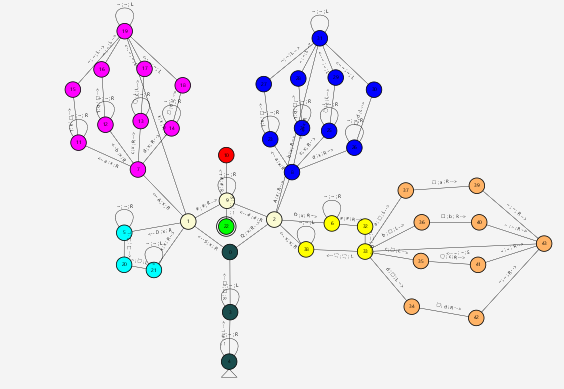
\includegraphics[width=\linewidth]{stackqueue.png}
    \caption{Turing Machine.}
    \label{fig:stackqueue}
\end{figure}

\section{Instructions}
A's mean to add the next character and D's mean to delete from the top or the bottom, depending on whether you specified a stack or a queue
by either inputting an S or Q at the beginning of the string. 
You can add a,b,c, or d. This can, of course, be implemented with any character,
but using only 4 characters makes it easier to visualize the states.

\section{Examples}
Here are some examples of input and output for the Turing machine:
\begin{itemize}
    \item \begin{verbatim} Input: SAaAbD, Output: xxxxxx#a \end{verbatim}
    \item \begin{verbatim} Input: SAaAbAcDAdAaDD, Output: xxxxxxxxxxxxx#ab \end{verbatim}
    \item \begin{verbatim} Input: QAaAbD, Output: xxxxxx#b \end{verbatim}
    \item \begin{verbatim} Input: QAaAbAcDAdAaDD, Output: xxxxxxxxxxxxx#da \end{verbatim}
    \item \begin{verbatim} Input: QA#AbD, Output: INVALID \end{verbatim}
    \item \begin{verbatim} Input: QA1A2D, Output: INVALID \end{verbatim}
\end{itemize}

\section{Conclusion}
The Turing machine is a powerful tool for performing computations on input tapes. It has applications in computer science, mathematics, and other fields.

\end{document}